\section{Технический проект}
\subsection{Общая характеристика организации решения задачи}

Программно-информационная система представляет собой современное веб-приложение, предназначенное для автоматизации управления книжным магазином. Система разработана с использованием модульной архитектуры, что позволяет легко адаптировать её к потребностям малого и среднего бизнеса, а также расширять функционал при необходимости.

В основе системы лежит серверная часть, реализованная на Flask с использованием RESTful API. Это обеспечивает быстрое и удобное взаимодействие между клиентской частью и сервером. Веб-интерфейс построен с использованием HTML, CSS и JavaScript, что делает систему доступной в любом современном браузере. База данных PostgreSQL выступает в качестве хранилища данных, а библиотека psycopg2 используется для взаимодействия с ней.

Система предоставляет удобные возможности для всех категорий пользователей. Покупатели могут просматривать каталог книг, использовать поиск, корзину для оформления заказов и отслеживать их статус. Также доступна страница книги с подробной информацией, включая описание и дополнительные характеристики.

Для сотрудников магазина предусмотрен интерфейс, позволяющий редактировать информацию о книгах, изменять их наличие, а также обновлять статусы заказов покупателей. Администраторы имеют доступ ко всему функционалу сотрудников, а также к управлению ролями пользователей. Это позволяет быстро изменять права доступа, добавлять новых сотрудников или ограничивать доступ к определённым функциям.

Система поддерживает аутентификацию и авторизацию пользователей, обеспечивая безопасное использование. Реализована возможность работы с несколькими ролями: покупатель, сотрудник и администратор, что делает её гибкой и подходящей для различных сценариев использования.

Ключевая особенность системы – её масштабируемость. Архитектура позволяет легко добавлять новые функции, такие как поддержка скидок, интеграция с платёжными системами или создание аналитических отчётов о продажах. Также предусмотрена возможность адаптации интерфейса под мобильные устройства, что обеспечивает доступность для пользователей с разных платформ.

Применение системы эффективно в книжных магазинах, где требуется централизованное управление ассортиментом и заказами. Её также можно модифицировать для других сфер розничной торговли. Перспективы развития включают добавление системы промокодов, расширение функционала аналитики и поддержку мультиязычного интерфейса, что сделает её полезным инструментом для международных пользователей.

Эта система сочетает простоту в использовании и высокую гибкость настройки, предоставляя удобные инструменты для управления книжным магазином.

\subsection{Обоснование выбора технологии проектирования}

Выбор технологий, языков программирования и архитектурных решений для реализации программно-информационной системы обусловлен совокупностью факторов, направленных на обеспечение высокой гибкости, надёжности и простоты сопровождения программного продукта. Используемые для создания программно-информационной системы языки и технологии отвечают современным практикам разработки, позволяют достичь высокой производительности и отказоустойчивости программы.

\subsubsection{Язык программирования Python}

В качестве языка программирования для серверной части выбран Python, благодаря его сочетанию выразительности, гибкости и обширной поддержки со стороны сообщества разработчиков. Python — это высокоуровневый, интерпретируемый язык, активно применяющийся как в образовательных, так и в промышленных проектах. Основные причины выбора языка заключаются в следующем:
\begin{enumerate}
	\item Простой и интуитивно понятный синтаксис значительно сокращает порог вхождения и снижает количество потенциальных ошибок при написании кода. Это особенно важно в условиях ограниченного времени на разработку и тестирование, а также при передаче проекта на сопровождение.
	\item Поддержка нескольких парадигм программирования, включая объектно-ориентированную, процедурную и функциональную, делает Python универсальным инструментом. Это позволяет организовать код в соответствии с принципами модульности, инкапсуляции и повторного использования.
	\item Обширная стандартная библиотека и внешняя экосистема обеспечивают доступ к готовым модулям для сериализации, построения интерфейса, анализа синтаксических деревьев, многопоточности и многого другого. Это существенно ускоряет разработку и упрощает реализацию сложных функций.
	\item Кроссплатформенность языка позволяет запускать приложение на операционных системах Windows, Linux и macOS без необходимости адаптации кода под конкретную платформу. Таким образом, обеспечивается максимальная универсальность и доступность системы для пользователя.	
\end{enumerate}


Таким образом, Python представляет собой оптимальное решение для реализации проекта, сочетающее в себе простоту, мощь и гибкость, что делает его незаменимым инструментом в учебных и практических задачах программной инженерии.

\subsubsection{Язык программирования JavaScript}

JavaScript был выбран в качестве основного языка клиентской части, так как он покрывает все необходимые требования поставленные в задаче. Главные преимущества языка для проекта заключается в следующем:
 
\begin{enumerate}
	\item JavaScript является единственным языком, который исполняется на стороне клиента без необходимости дополнительных компиляторов или плагинов. Все современные браузеры (Chrome, Firefox, Safari, Edge) имеют возможность его выполнения.
	\item Интерактивность без перезагрузки страницы. Приложение книжного магазина требует динамического обновления корзины, каталога и форм без перезагрузки страницы, что позволяет реализовывать JavaScript.
	\item Работа с локальным хранилищем для хранения корзины пользователей.
	\item Событийно-ориентированная модель для обработки действия пользователя.
	\item Интеграция с внешними API для взаимодействия с Flask.
\end{enumerate}

\subsubsection{Фреймворк Flask}

Для реализации серверной части REST API выбран фреймворк Flask, основанный на Python. Flask — это легковесный, но мощный веб-фреймворк, который идеально подходит для создания масштабируемых и гибких веб-приложений. Его выбор обоснован следующими преимуществами:
\begin{enumerate}
	\item Предоставляет только базовые инструменты для разработки веб-приложений, позволяя разработчику выбирать дополнительные библиотеки и подходы. Это упрощает настройку REST API под конкретные задачи книжного магазина, такие как управление каталогом, заказами и пользователями.
	\item Легко интегрируется с библиотекой psycopg2 для работы с PostgreSQL, что обеспечивает эффективное взаимодействие с базой данных. Также поддерживаются модули для аутентификации и авторизации, что важно для управления ролями (покупатель, сотрудник, администратор).
	\item Позволяет быстро создавать эндпоинты для обработки HTTP-запросов, что соответствует архитектуре REST, используемой в системе.
	\item Благодаря легковесной архитектуре Flask минимизирует накладные расходы, обеспечивая быструю обработку запросов, что критично для веб-приложения с большим количеством пользователей.
\end{enumerate}

Flask выбран как основа серверной части благодаря своей простоте, гибкости и способности эффективно решать задачи, связанные с созданием REST API для книжного магазина.

\subsubsection{Графический интерфейс с использованием HTML и CSS}

Для создания графического интерфейса выбраны HTML и CSS, обеспечивающие структуру и оформление веб-страниц.

HTML используется для разметки страниц, определяя структуру элементов (каталог книг, корзина, формы).
Основные преимущества использования HTML:
\begin{enumerate}
	\item Простота и универсальность, позволяющие быстро создавать структурированные страницы.
	\item Поддержка всеми браузерами, гарантирующая кросс-браузерную совместимость.
	\item Гибкость в создании элементов интерфейса, таких как карточки книг и формы заказа.
\end{enumerate}

CSS отвечает за стилизацию интерфейса, включая цвета, шрифты и расположение элементов.
Основные преимущества использования CSS:
\begin{enumerate}
	\item Возможность создания адаптивного дизайна с помощью медиа-запросов для поддержки разных устройств (компьютеры, смартфоны, планшеты).
	\item Разделение структуры (HTML) и оформления (CSS) упрощает поддержку и обновление интерфейса.
	\item Поддержка анимаций и переходов для улучшения пользовательского опыта.
\end{enumerate}


Выбор HTML и CSS обоснован их стандартизацией, простотой и способностью создавать адаптивный и функциональный интерфейс, соответствующий требованиям книжного магазина.


\subsection{Архитектура программной системы}

 На рисунке 3.1 в виде UML-диаграммы представлена архитектура
программной системы.

\begin{figure}[H]
	\centering
	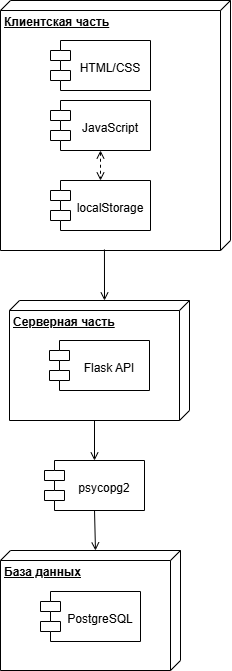
\includegraphics[width=0.3\linewidth]{images/диаграмма_компонентов}
	\caption{}
	\label{fig:}
\end{figure}


Программно-информационная система книжного магазина состоит из следующих компонентов:

\begin{enumerate}
	\item Клиентская часть: одностраничное приложение, работающее в браузере пользователя, реализованное с использованием HTML, CSS для интерфейса и JavaScript для динамической обработки данных, включая взаимодействие с сервером и временное хранение данных в localStorage. 
	\item Серверная часть: REST API сервер, разработанный на Python с использованием Flask, обеспечивающий управление каталогом книг, обработку заказов, аутентификацию и авторизацию пользователей, а также ролями (покупатель, сотрудник, администратор).
	\item База данных: реляционная СУБД PostgreSQL, хранящая данные о книгах, авторах, жанрах, пользователях и заказах, взаимодействующая с серверной частью через библиотеку psycopg2. 
\end{enumerate}

\subsection{Проект данных программной системы}

В рамках разработанной программной системы книжного магазина используется реляционная база данных PostgreSQL, которая обеспечивает надежное хранение и обработку структурированных данных. PostgreSQL была выбрана как мощная и надежная система управления базами данных с открытым исходным кодом, поддерживающая все необходимые функции для данного проекта. На стороне клиента для хранения временных данных, таких как содержимое корзины и информация о текущем пользователе, применяется механизм localStorage, встроенный в современные веб-браузеры. PostgreSQL представляет собой традиционную SQL-базу данных, которая хранит информацию в виде таблиц со строго определенной структурой, что обеспечивает целостность данных и позволяет выполнять сложные запросы с соединениями таблиц.

Для взаимодействия с PostgreSQL из Python-приложения используется библиотека psycopg2, которая предоставляет удобный интерфейс для выполнения SQL-запросов и работы с результатами. На клиентской стороне localStorage, хотя и не является полноценной базой данных, обеспечивает простой и эффективный способ хранения информации непосредственно в браузере пользователя без необходимости установки дополнительного программного обеспечения. Такой подход позволяет сохранять состояние приложения между сеансами работы, например, содержимое корзины или данные авторизации, при этом не требуя сложной синхронизации с сервером. Выбор именно этой архитектуры хранения данных обусловлен относительной простотой системы, отсутствием необходимости в горизонтальном масштабировании и четко определенной структурой данных, характерной для предметной области интернет-магазина книг.

Комбинация PostgreSQL на сервере и localStorage на клиенте представляет собой оптимальное решение для данного проекта, обеспечивая как надежность и структурированность хранения основных данных, так и гибкость работы с временной информацией на стороне клиента.

\subsubsection{Описание сущностей}

 В таблице 3.1 приведен набор полей JSON-документа и их описание для сущности «Авторы».

\begin{xltabular}{\textwidth}{|c|c|X|}
	\caption{Описание сущности "Авторы"\label{authors:table}}\\ \hline
	\thead{Ключ} & \thead{Тип} & \thead{Описание} \\ \hline
	\endfirsthead
	\continuecaption{Продолжение таблицы \ref{authors:table}}\\ \hline
	\thead{Ключ} & \thead{Тип} & \thead{Описание} \\ \hline
	\endhead
	id & integer & Уникальный идентификатор автора (первичный ключ) \\ \hline
	name & varchar(100) & Полное имя автора \\ \hline
\end{xltabular}

 В таблице 3.2 приведен набор полей JSON-документа и их описание для сущности «Жанры».
 
\begin{xltabular}{\textwidth}{|c|c|X|}
	\caption{Описание сущности "Жанры"\label{genres:table}}\\ \hline
	\thead{Ключ} & \thead{Тип} & \thead{Описание} \\ \hline
	\endfirsthead
	\continuecaption{Продолжение таблицы \ref{genres:table}}\\ \hline
	\thead{Ключ} & \thead{Тип} & \thead{Описание} \\ \hline
	\endhead
	id & integer & Уникальный идентификатор жанра (первичный ключ) \\ \hline
	name & varchar(50) & Название жанра (уникальное) \\ \hline
\end{xltabular}

 В таблице 3.3 приведен набор полей JSON-документа и их описание для сущности «Книги».
 
\begin{xltabular}{\textwidth}{|c|c|X|}
	\caption{Описание сущности "Книги"\label{books:table}} \\ \hline
	\thead{Ключ} & \thead{Тип} & \thead{Описание} \\ \hline
	\endfirsthead
	\caption*{Продолжение таблицы \ref{books:table}} \\ \hline
	\thead{Ключ} & \thead{Тип} & \thead{Описание} \\ \hline
	\endhead
	id & integer & Уникальный идентификатор книги (первичный ключ) \\ \hline
	title & varchar(200) & Название книги \\ \hline
	author\_id & integer & Внешний ключ, ссылается на таблицу авторов \\ \hline
	genre\_id & integer & Внешний ключ, ссылается на таблицу жанров \\ \hline
	price & numeric(10,2) & Цена книги \\ \hline
	description & text & Описание книги (может быть NULL) \\ \hline
	quantity\_in\_stock & integer & Количество экземпляров на складе \\ \hline
	sold\_copies & integer & Количество проданных экземпляров \\ \hline
	publication\_date & date & Дата публикации (может быть NULL) \\ \hline
	created\_at & timestamp & Дата и время добавления книги \\ \hline
\end{xltabular}

 В таблице 3.4 приведен набор полей JSON-документа и их описание для сущности «Пользователи».
 
\begin{xltabular}{\textwidth}{|c|c|X|}
	\caption{Описание сущности "Пользователи"\label{users:table}}\\ \hline
	\thead{Ключ} & \thead{Тип} & \thead{Описание} \\ \hline
	\endfirsthead
	\continuecaption{Продолжение таблицы \ref{users:table}}\\ \hline
	\thead{Ключ} & \thead{Тип} & \thead{Описание} \\ \hline
	\endhead
	id & integer & Уникальный идентификатор пользователя (первичный ключ) \\ \hline
	username & varchar(50) & Логин пользователя (уникальный) \\ \hline
	email & varchar(100) & Email пользователя (уникальный, может быть NULL) \\ \hline
	password & text & Пароль пользователя \\ \hline
	role & varchar(20) & Роль: customer, employee, admin \\ \hline
	created\_at & timestamp & Дата и время регистрации \\ \hline
\end{xltabular}

 В таблице 3.5 приведен набор полей JSON-документа и их описание для сущности «Заказы».
 
\begin{xltabular}{\textwidth}{|c|c|X|}
	\caption{Описание сущности "Заказы"\label{orders:table}} \\ \hline
	\thead{Ключ} & \thead{Тип} & \thead{Описание} \\ \hline
	\endfirsthead
	
	\caption*{Продолжение таблицы \ref{orders:table}} \\ \hline
	\thead{Ключ} & \thead{Тип} & \thead{Описание} \\ \hline
	\endhead
	
	id & integer & Уникальный идентификатор заказа (первичный ключ) \\ \hline
	user\_id & integer & Внешний ключ, ссылается на таблицу пользователей \\ \hline
	order\_date & timestamp & Дата и время оформления заказа \\ \hline
	total\_amount & numeric(10,2) & Общая сумма заказа \\ \hline
	status & varchar(20) & Статус: processing, shipped, delivered, cancelled \\ \hline
\end{xltabular}
 В таблице 3.6 приведен набор полей JSON-документа и их описание для сущности «Элементы заказа».
 
\begin{xltabular}{\textwidth}{|c|c|X|}
	\caption{Описание сущности "Элементы заказа"\label{order_items:table}}\\ \hline
	\thead{Ключ} & \thead{Тип} & \thead{Описание} \\ \hline
	\endfirsthead
	\continuecaption{Продолжение таблицы \ref{order_items:table}}\\ \hline
	\thead{Ключ} & \thead{Тип} & \thead{Описание} \\ \hline
	\endhead
	id & integer & Уникальный идентификатор элемента заказа (первичный ключ) \\ \hline
	order\_id & integer & Внешний ключ, ссылается на таблицу заказов \\ \hline
	book\_id & integer & Внешний ключ, ссылается на таблицу книг \\ \hline
	quantity & integer & Количество экземпляров книги в заказе \\ \hline
	price\_at\_purchase & numeric(10,2) & Цена книги на момент покупки \\ \hline
\end{xltabular}

\subsection{Проектирование пользовательского интерфейса}

На основании требований к пользовательскому интерфейсу, представленных в пункте 2.3.3 технического задания, был разработан графический интерфейс программно-информационной системы управления книжным магазином. Для создания пользовательского интерфейса используется разметка, основанная на HTML и CSS.

На рисунке 3.1 представлен макет интерфейса главной страницы. Макет содержит следующие элементы:
\begin{enumerate}
	\item Поисковая строка.
	\item Карточка книги.
	\item Название книги.
	\item Автор книги.
	\item Цена книги.
	\item Количество на складе.
	\item Кнопка открывающая модальное окно с  подробным описанием книги.
	\item Кнопка добавляющая выбранную книгу в корзину.
	\item Кнопка открывающая модальное окно с авторизацией и регистрацией.
	\item Пагинация.
\end{enumerate}

\begin{figure}[H]
	\centering
	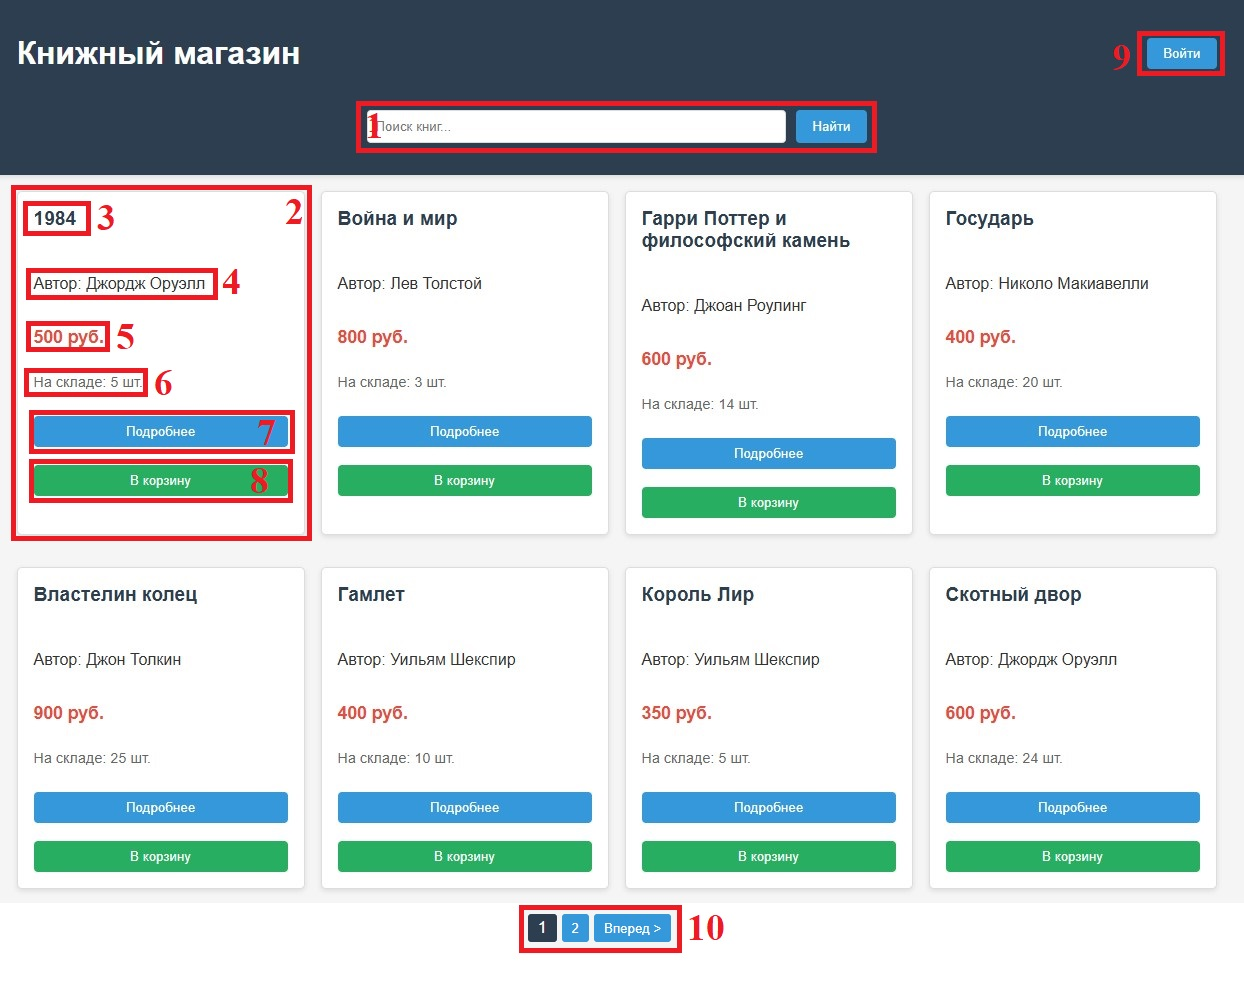
\includegraphics[width=0.7\linewidth]{images/Главная_страница}
	\caption{Макет интерфейса главной страницы}
	\label{fig:}
\end{figure}

На рисунке 3.2 представлен макет интерфейса корзины. Макет содержит следующие элементы:

\begin{enumerate}
	\item Книга добавленная пользователем в корзину.
	\item Количество и кнопки для изменения количества конкретной книги в корзине.
	\item Наименование книги.
	\item Суммарная стоимость выбранного количества книг одного наименования.
	\item Кнопка удаления книг одного наименования из корзины.
	\item Кнопка для оформления заказа.
	\item Итоговая стоимость книг в корзине.
\end{enumerate}

\begin{figure}[H]
	\centering
	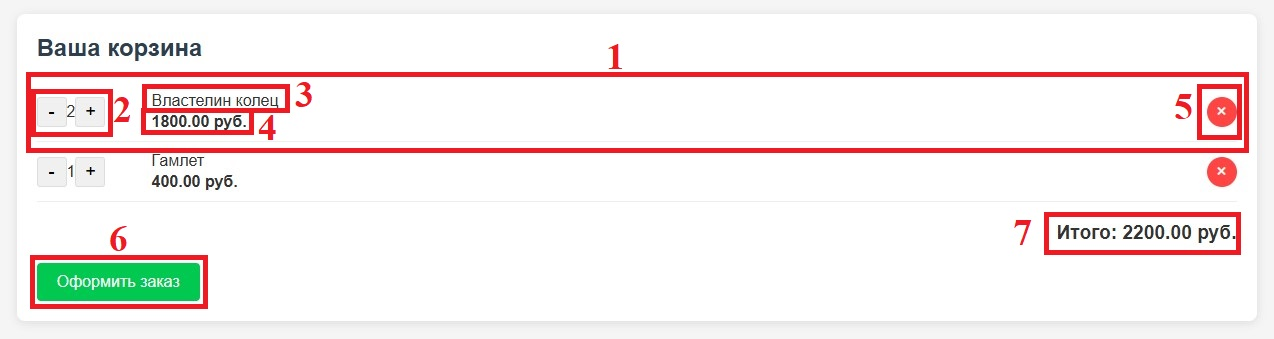
\includegraphics[width=0.7\linewidth]{images/Корзина}
	\caption{Макет интерфейса корзины}
	\label{fig:}
\end{figure}

На рисунке 3.3 представлен макет панели администратора. Макет содержит следующие элементы:

\begin{enumerate}
	\item Поле ввода для имени пользователя.
	\item Выпадающий список с выбором роли.
	\item Кнопка применения роли для выбраного пользователя.
	\item Кнопка актуализации данных списка пользователей.
	\item Список всех учётных записей и их данных.
	\item Кнопка для перехода к форме добавления книги.
\end{enumerate}

\begin{figure}[H]
	\centering
	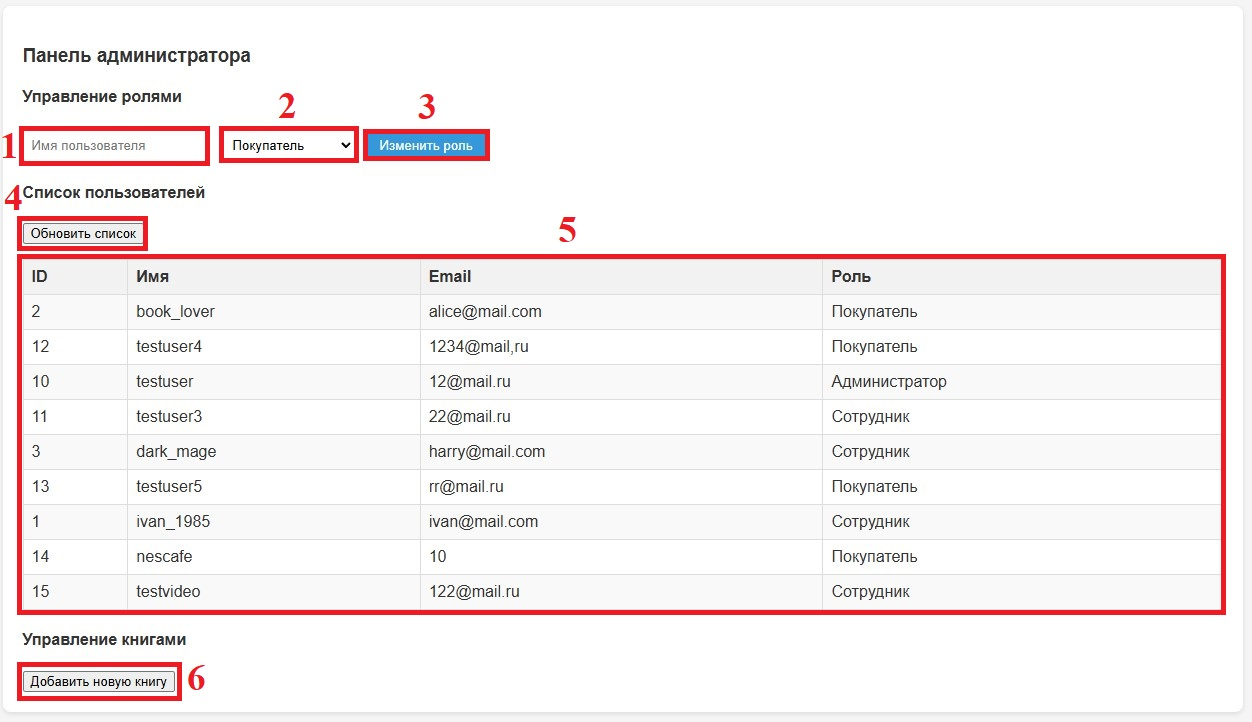
\includegraphics[width=0.7\linewidth]{images/Панель_администратора}
	\caption{Макет интерфейса панели администратора}
	\label{fig:}
\end{figure}

